\section{Results Overview}
\label{sec:overview}

In this section, the main goal is to overview the results not in terms of their scientific contribution but in terms of their bibliographic data for presenting an overview of the included records in the review. First, statistic results of the data sources in which the 142 included records could be identified in the methodology allow the evaluation of the coverage between the sources.
Next, the tool VOSviewer~\parencite{results:vosviewer:1,results:vosviewer:2} is used to obtain the co-occurrence analysis for the keywords and the authors. The former focus on the keywords recency and their occurrence in the sources, while the latter discusses the research networks between the authors, and the ones with more publications in long-term localization and mapping.
Lastly, two analysis are presented relative to the evolution of the publication year and most relevant publication venues.

\subsection{Data source}
\label{sec:overview:db}

The results on the identification phase are exported to BibTeX files from each data source. This exportation considers all the information available in the data sources, such as citation (e.g., author, title, publication venue, and type of record) and bibliographic (e.g., affiliation and the publisher) information of each record, the abstract, and author and indexed keywords. Next, using the \texttt{bibtexparser}\footnote{\url{https://bibtexparser.readthedocs.io/en/master/}} Python library, the BibTeX files are processed to identify uncompleted records. For example, the DOI must be specified and, if not available, the record's information must be manually completed with a corresponding URL. Then, considering the 142 included records in this review, a Python script searches each record in the BibTeX files corresponding to each data source. This search uses the DOI, URL, and title data to identify if a data source had in its identification results the searched record. Given that these three fields can contain lower and upper letters, the respective strings must be compared only after converting them to lower cases. As a result, the number of identified records by each data source of the 142 included ones in the review are the following ones:

\begin{itemize}[nosep]
\item \citetitle{methodology:search:db:acm}: 25 records (17.6\%);
\item \citetitle{methodology:search:db:dimensions}: 84 records (59.2\%);
\item \citetitle{methodology:search:db:ieee-xplore}: 67 records (47.2\%);
\item \citetitle{methodology:search:db:inspec}: 102 records (71.8\%);
\item \citetitle{methodology:search:db:scopus}: 120 records (84.5\%);
\item \citetitle{methodology:search:db:wos}: 105 records (73.9\%).
\end{itemize}

The database \citetitle{methodology:search:db:scopus} is the source that identified the greatest number of included records. This result was expected given that \citetitle{methodology:search:db:scopus} is considered as one of the largest curated databases~\parencite{methodology:search:db:coverage:dim-scopus-wos}, indexing more than 25000 active titles (e.g., conferences proceedings, journals) and 7000 publishers\footnote{\url{https://www.elsevier.com/solutions/scopus/how-scopus-works}}.
Two other sources with more than 70\% of identified records are \citetitle{methodology:search:db:inspec} and \citetitle{methodology:search:db:wos}. Similarly to \citetitle{methodology:search:db:scopus}, these two databases index also records from thousands of journals, conferences, and publishers\footnote{\url{https://www.elsevier.com/solutions/engineering-village/content/inspec}}\textsuperscript{,}\footnote{\url{https://clarivate.com/webofsciencegroup/solutions/web-of-science/}}.
Although \citetitle{methodology:search:db:dimensions} is also a bibliographic database covering millions of publications from thousands of sources, this database is the newest one (created in 2018) relative to the other three considered in this review (\citetitle{methodology:search:db:inspec}, \citetitle{methodology:search:db:scopus}, and \citetitle{methodology:search:db:wos}) and could be a factor to why it obtained a lower percentage (59.2\%) than the other three databases. Another possible reason is that \citetitle{methodology:search:db:scopus} and \citetitle{methodology:search:db:wos} have the majority of their coverage in Life Sciences, Physical Sciences, and Technology Area (including the Engineering subject area related to the topic of this review), while \citetitle{methodology:search:db:dimensions} has better coverage in Social Sciences and Arts \& Humanities~\parencite{methodology:search:db:coverage:dim-scopus-wos}.
Even though \citetitle{methodology:search:db:ieee-xplore} is a digital library and only indexes works published by IEEE and its partners, this data source returns 47.2\% of the include records in the review. The main reason is that this library indexes publications related to electrical engineering and computer science, subject areas related to long-term localization and mapping\footnote{\url{https://ieeexplore.ieee.org/Xplorehelp/overview-of-ieee-xplore/about-ieee-xplore}}.
Finally, the \citetitle{methodology:search:db:acm} using \textit{The ACM Guide to Computing Literature} collection only finds published records by ACM and possible links to other records focused exclusively on computing\footnote{\url{https://libraries.acm.org/digital-library/acm-guide-to-computing-literature}} and not directly related to the Computer Science or Engineering subject areas, explaining why this source obtained a lower coverage percentage of the included results than the other sources for this review.

Furthermore, Table~\ref{tab:overview:source} presents a coverage analysis of the identified results from each data source for the 142 included records in this review. Table~\ref{tab:overview:source:intersect} presents the pairwise overlap between sources. The corresponding percentage is the ratio of records identified by both sources to the one between the two that has the smallest number of results: $\#\{A\cap B\} / \text{min}\{\#A,\#B\}$, where $\#A$ and $\#B$ is the number of results for a data source $A$ and $B$, respectively, and $\#\{A\cap B\}$ is the intersection results between the two sources. For example, if the pairwise results is 100\%, it means that the data source with more records found was capable of obtaining all the results, i.e., had full coverage over the other source. Table~\ref{tab:overview:source:union} reports the percentage of records identified by at least one of two data sources over all 142 included records: $\#\{A\cup B\} / 142$, where $A\cup B$ is the union correspondence results of the sources $A$ and $B$. This percentage represents the joint coverage of two databases over the 142 included records.
					
\begin{table}[h]
  \centering
  \caption{Pairwise coverage analysis of the data sources considered in the review over the 142 included records: (a) identification only on both pairwise sources ($\#\{A\cap B\} / \text{min}\{\#A,\#B\}$); (b) on either ones ($\#\{A\cup B\} / \#\text{records}$). Legend: dim -- \citetitle{methodology:search:db:dimensions}, ieee -- \citetitle{methodology:search:db:ieee-xplore}, insp -- \citetitle{methodology:search:db:inspec}, scop -- \citetitle{methodology:search:db:scopus}, wos -- \citetitle{methodology:search:db:wos}.}
  \label{tab:overview:source}
  \subfloat[][]{%
  \label{tab:overview:source:intersect}%
  \begin{tabular}{l|P{0.08\columnwidth}P{0.08\columnwidth}P{0.08\columnwidth}P{0.08\columnwidth}P{0.08\columnwidth}P{0.08\columnwidth}}
\hline
$A\cap B$ & \textbf{acm} & \textbf{dim} & \textbf{ieee} & \textbf{insp} & \textbf{scop} & \textbf{wos}\\
\hline
\textbf{acm}  & -- & 96.0\% & 44.0\% & 88.0\% & 96.0\% & 96.0\%\\
\textbf{dim}  & -- & --     & 68.7\% & 77.4\% & 97.6\% & 96.4\%\\
\textbf{ieee} & -- & --     & --     & 89.6\% & 91.0\% & 74.6\%\\
\textbf{insp} & -- & --     & --     & --     & 87.3\% & 69.6\%\\
\textbf{scp}  & -- & --     & --     & --     & --     & 89.5\%\\
\textbf{wos}  & -- & --     & --     & --     & --     & --\\
\hline
    \end{tabular}%
  }
  \linebreak
  \subfloat[][]{%
  \label{tab:overview:source:union}%
  \vspace{0.5em}
  \begin{tabular}{l|P{0.08\columnwidth}P{0.08\columnwidth}P{0.08\columnwidth}P{0.08\columnwidth}P{0.08\columnwidth}P{0.08\columnwidth}}
\hline
$A\cup B$ & \textbf{acm} & \textbf{dim} & \textbf{ieee} & \textbf{insp} & \textbf{scop} & \textbf{wos}\\
\hline
\textbf{acm}  & -- & 59.9\% & 57.0\% & 73.9\% & 85.2\% & 74.6\%\\
\textbf{dim}  & -- & --     & 73.9\% & 85.2\% & 85.9\% & 76.1\%\\
\textbf{ieee} & -- & --     & --     & 76.8\% & 88.7\% & 85.9\%\\
\textbf{insp} & -- & --     & --     & --     & 93.7\% & 95.8\%\\
\textbf{scp}  & -- & --     & --     & --     & --     & 92.3\%\\
\textbf{wos}  & -- & --     & --     & --     & --     & --\\
\hline
  \end{tabular}%
  }
\end{table}

Analyzing the coverage results in Table~\ref{tab:overview:source}, the first observation is that the pairwise union results of two sources increase the independent coverage of each source. This observation validates the need identified in the methodology discussed in Section~\ref{sec:methodology} to consider several data sources in the identification phase of a review. Moreover, the pairwise union coverage of \citetitle{methodology:search:db:inspec}, \citetitle{methodology:search:db:scopus}, and \citetitle{methodology:search:db:wos} is greater than 90\% of the included records. When evaluating the joint coverage of these three databases, they identify all 142 of the included records, i.e., a 100\% coverage. Although this result could indicate that those three sources guarantee full coverage of the long-term localization and mapping research topic, it is always advisable to consider as most as possible sources in the methodology. Another observation is relative to the overlap of \citetitle{methodology:search:db:scopus} with the other sources, which is greater than 85\%. This overlap indicates that \citetitle{methodology:search:db:scopus} covers results not only on the topic of this review but also the results obtained by the other sources considered in the methodology. Lastly, \citetitle{methodology:search:db:inspec} and \citetitle{methodology:search:db:wos} achieve a pairwise overlap percentage of 69.6\% between themselves, while their union represents 95.8\% of the included records. This discrepancy indicates that these two sources identify unique results between themselves. Indeed, \citetitle{methodology:search:db:inspec} identifies 31/142 records not found by \citetitle{methodology:search:db:wos}, and vice-versa for \citetitle{methodology:search:db:wos}, with 34/142 unique records.

\subsection{Keywords co-occurrence}
\label{sec:overview:kw}

Next, VOSviewer~\parencite{results:vosviewer:1,results:vosviewer:2} is used to analyze the co-occurrence of keywords in the included articles. This co-occurrence is the relatedness of items determined based on the number of documents in which the keywords occur together.
For this analysis, first, a Python script processes the BibTeX file containing the citation and bibliographic information, the author and the indexed keywords, and the abstract of the records to join the author with the indexed keywords in the same \texttt{keywords} field. Then, an online tool\footnote{\url{https://www.bibtex.com/c/bibtex-to-ris-converter/}} converts this processed BibTeX to a RIS file.
Even though VOSviewer supports file types directly exported from \citetitle{methodology:search:db:dimensions}, \citetitle{methodology:search:db:scopus}, or \citetitle{methodology:search:db:wos} as input, none of these data sources obtained all the 142 included records of the review in the identification phase. Given that VOSviewer does not support BibTeX files, the conversion to RIS file is required for using as input.
The disadvantage of using this file format in VOSviewer is only allowing to perform co-occurrence of items (e.g., keywords or authors), while bibliographic data from \citetitle{methodology:search:db:dimensions}, \citetitle{methodology:search:db:scopus}, or \citetitle{methodology:search:db:wos} in CSV files would allow other analysis such as citation, co-citation, or bibliographic coupling.
However, the creation of these CSV files follow different templates depending on the data source. So, RIS files allow the integration of all 142 included records for obtaining the two co-occurrence analysis presented in this review (namely, keywords and co-authorship).

In Figure~\ref{fig:overview:kw:original}, the network presents the overlay visualization of the keywords co-occurrence in the included records weighted by the number of occurrences of each term, using full counting for the links' strength. The latter computes the strength of the links directly by the number of co-occurrences of the respective two terms.
The overlay visualization colors the keywords differently according to the average publication year of the included records in which each of the keywords appears. This coloring allows analyzing which are the ones that are associated with the most recent publications.
As for the keywords' weighting, the number of occurrences dictates the size of the circles.
Furthermore, the minimum number of occurrences of a keywords set in VOSviewer for obtaining the graph is 5 originating the 35 keywords illustrated in Figure~\ref{fig:overview:kw:original}. This parameter was selected for visualization purposes while also filtering uninteresting keywords.
Similarly, setting the attraction and repulsion parameters to 2 and 0, respectively, distances the terms more from each other than using the values recommended in the VOSviewer manual\footnote{\url{https://www.vosviewer.com/documentation/Manual_VOSviewer_1.6.8.pdf}} (2 and 1, respectively). These two parameters only interfere in the localization of the terms in the map, not in the graph connections.
Lastly, a thesaurus of the keywords (available in the repository) is used to join similar terms: spelling differences (e.g., localization -- localisation), full terms versus abbreviations (simultaneous localization and mapping -- SLAM), while also allowing the concatenation of long keywords for visualization reasons.

\begin{figure*}[!t]
  \centering
  \subfloat[][]{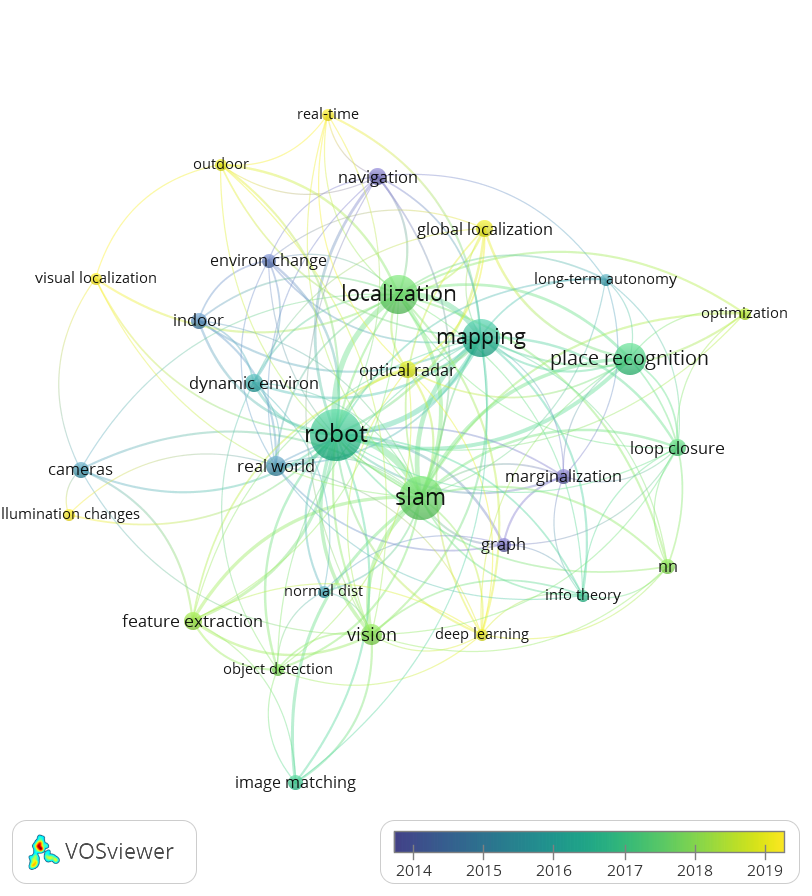
\includegraphics[width=\columnwidth]{figures/kw.png}%
  \label{fig:overview:kw:original}}
  \hfill
  \subfloat[][]{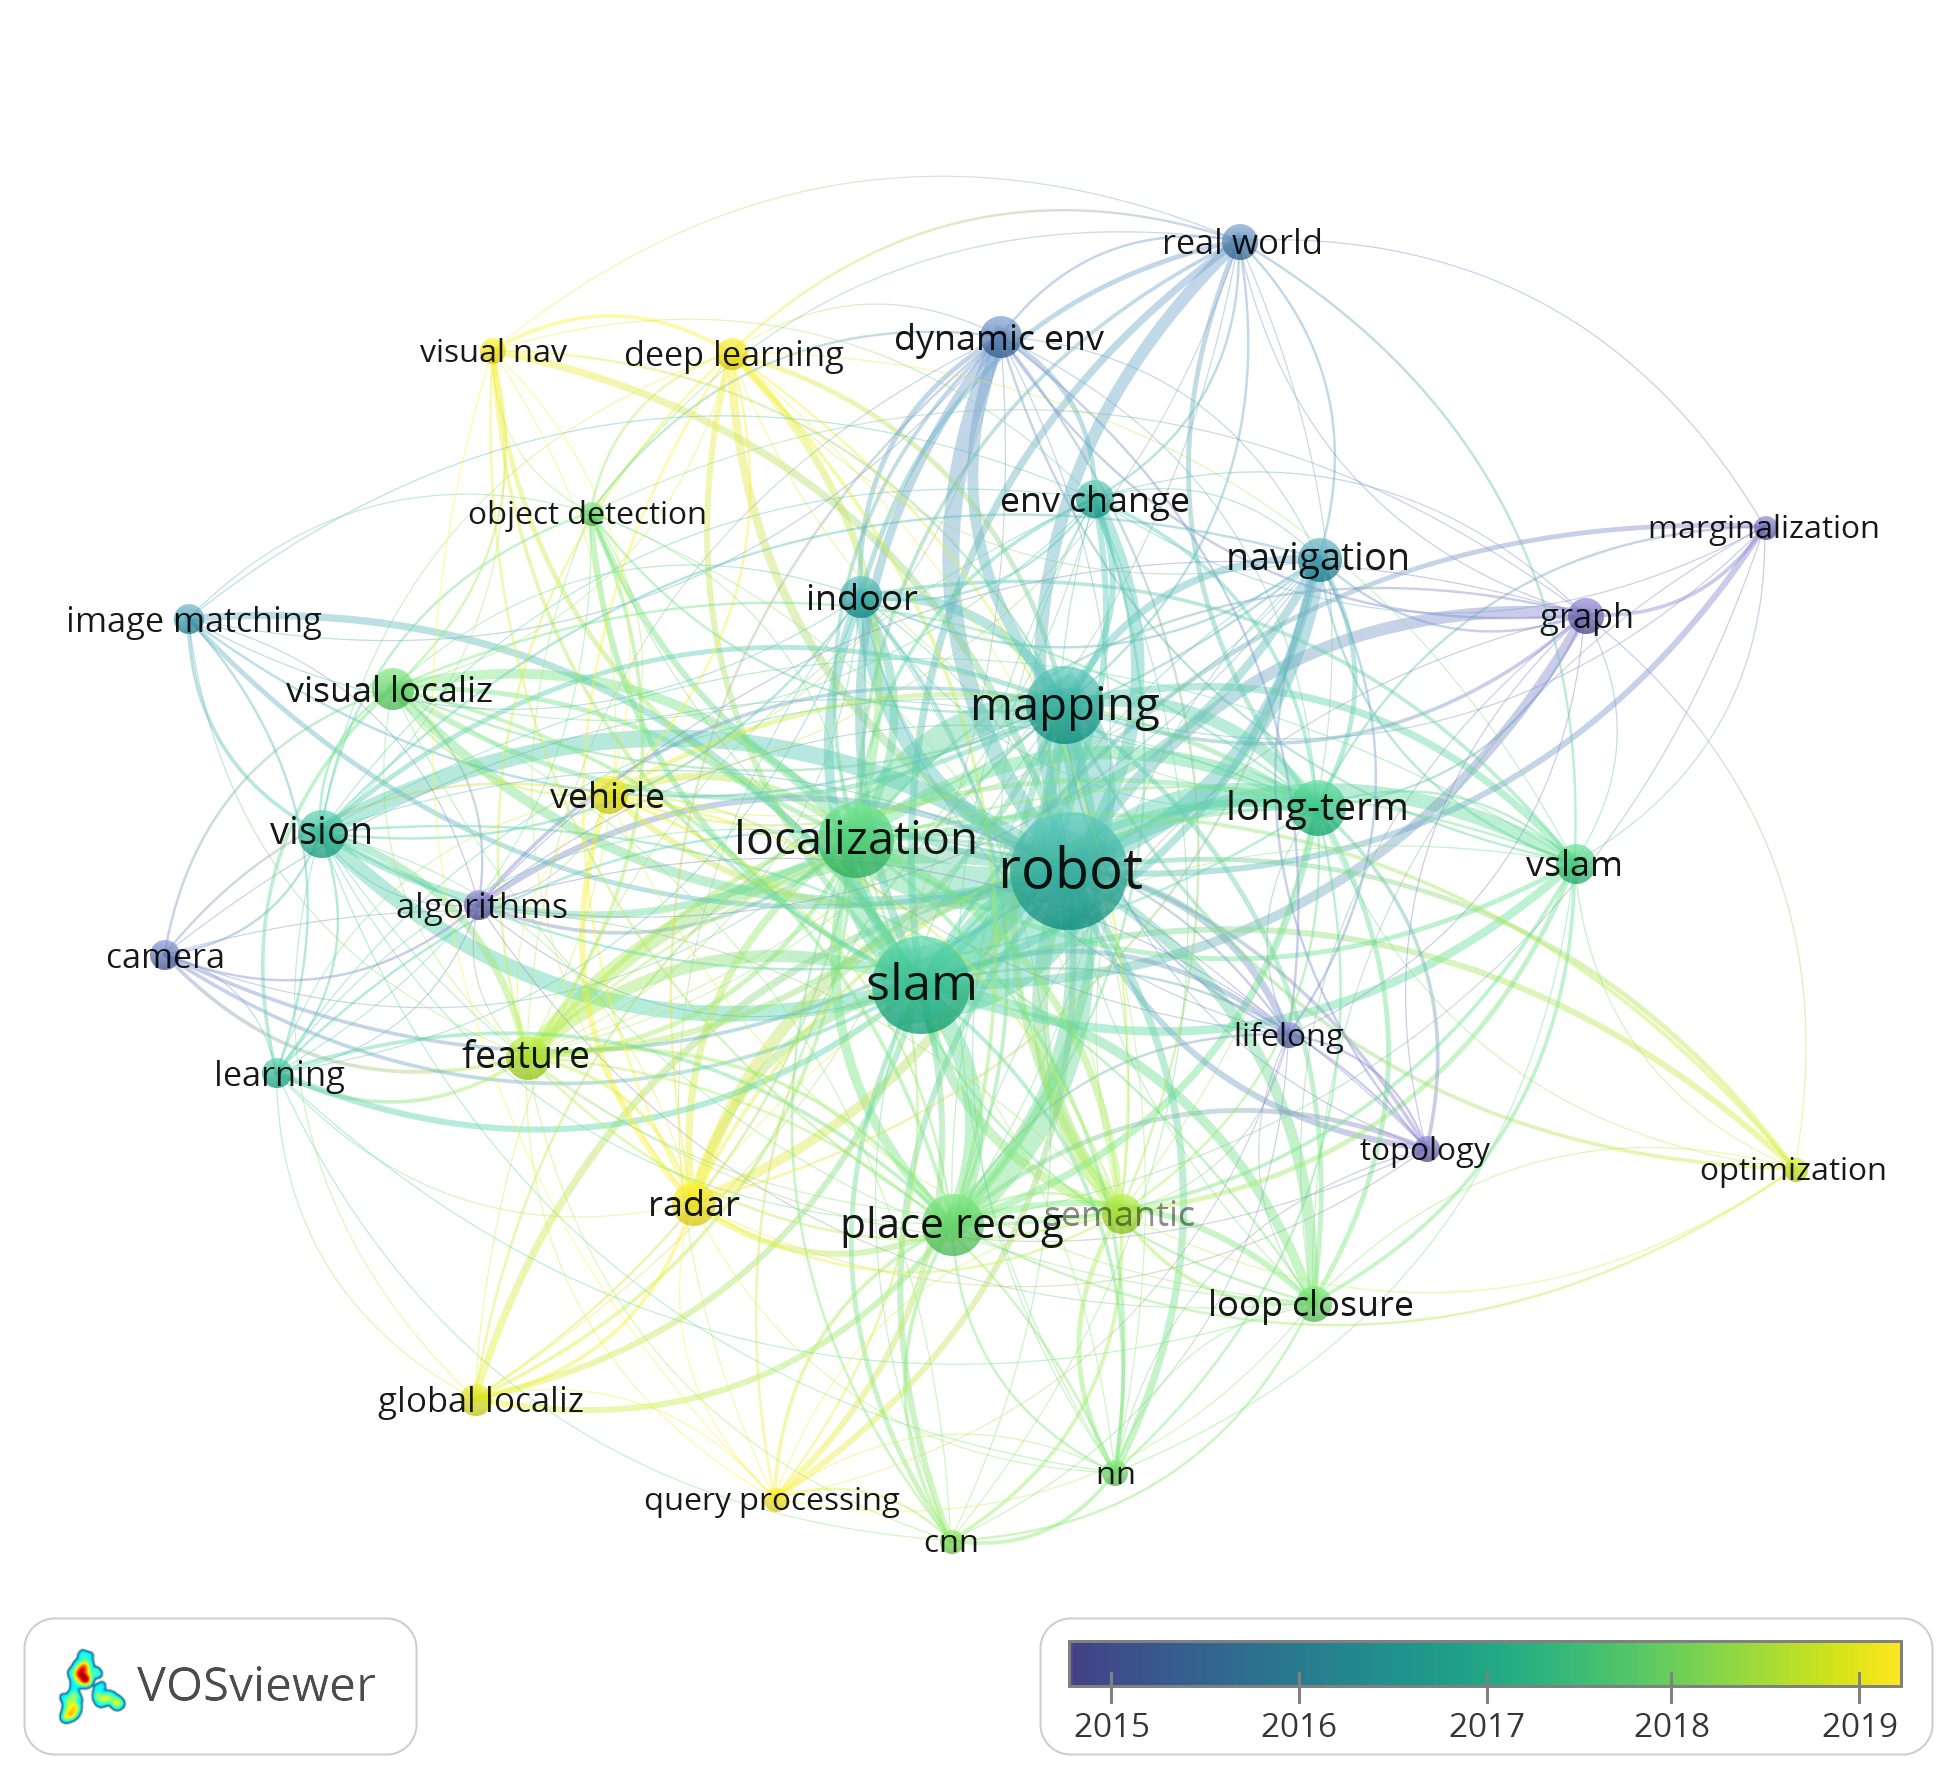
\includegraphics[width=\columnwidth]{figures/kw_long-term.png}%
  \label{fig:overview:kw:long-term}}
  \caption{Keywords co-occurrence analysis on the 142 included records generated by VOSviewer with overlay visualization by the average publication year: (a) original keywords; (b) all keywords containing long-term and lifelong summarized by the terms themselves. Parameters used for generating the co-occurrence network: minimum number of occurrences = 5, attraction = 2, repulsion = 0, scale = 1.49, circles size variation = 0.5, lines size validation = 1.0. Legend: \texttt{cnn} -- Convolutional Neural Networks, \texttt{env} -- environment, \texttt{localiz} -- localization, \texttt{nav} -- navigation, \texttt{nn} -- Neural Networks, \texttt{recog} -- recognition, \texttt{vslam} -- visual SLAM.}
  \label{fig:overview:kw}
\end{figure*}

Overall, the keyword \texttt{robot} is the one that appears more times in the included records: 111 occurrences, links with 34 other terms, and has a total link strength of 403 (sum of co-occurrences of all of its links). This result is expected due to the relation of this review's topic to robotics.
Similarly, three other keywords in the network related to long-term localization and mapping topic with high values of occurrence, number of links, and total link strength are \texttt{slam} (75, 34, and 288), \texttt{mapping} (48, 33, and 204), and \texttt{localization} (47, 32, and 194, respectively). The methodology for the search strategy discussed in Section~\ref{sec:methodology:search} considers all of these four keywords. Thus, the significant influence of \texttt{robot}, \texttt{slam}, \texttt{mapping}, and \texttt{localization} in the keywords co-occurrence analysis indicates that, after the all the phases executed in this review's methodology, the 142 included records have a high correlation with the keywords considered in the search query. Given that the keywords are usually selected or indexed to capture the essence of the document, this correlation indicates that the search query is appropriate to obtain the search results, even considering only the keywords as search fields.

As for keywords related to the outcome of the PICO framework, \texttt{long-term autonomy} occurs only 6 times in the included records, linking with 16 other keywords and having a total link strength of 27. This low occurrence could indicate that the term \texttt{long-term autonomy} is not usually used by the authors nor indexed by the databases. 
However, the specific term of \texttt{long-term autonomy} does not summarize all the possibilities for the outcome of the PICO framework (see Section~\ref{sec:purpose}). Indeed, for this reason, the search query for the identification phase uses only the following single terms: \texttt{"long term"} and \texttt{"life long"} (resumes the possibility of having a space or a hyphen), and \texttt{lifelong}.
Figure~\ref{fig:overview:kw:long-term} presents the keywords co-occurrence analysis using the same parameters for obtaining Figure~\ref{fig:overview:kw:original}. The difference to the latter network is using a thesaurus that summarizes all the keywords that contain \texttt{long-term} and \texttt{lifelong} into the terms themselves, obtaining 36 keywords with a minimum of 5 occurrences in the 142 included records.
In terms of occurrences, number of links, and total link strength, the impact of the thesaurus keyword \texttt{long-term} is 25, 28, and 105, and for lifelong 6, 17, and 31, respectively. These values are much higher than the ones respective only to \texttt{long-term autonomy} from Figure~\ref{fig:overview:kw:original}.
The reason is that \texttt{long-term} in Figure~\ref{fig:overview:kw:long-term} compiles the occurrences of keywords such as \texttt{long-term autonomy}, \texttt{long-term mapping}, and \texttt{long-term localization} (6, 2, and 2 occurrences, respectively), and \texttt{lifelong} sum up, for example, three different versions of \texttt{lifelong learning} (using \texttt{lifelong}, \texttt{life-long} and \texttt{life long} with 2, 1, and 2 occurrences, respectively) and \texttt{lifelong slam} (1 occurrence). Hence, these results proves that the third \texttt{AND} part of the search query (\texttt{"long term" OR "life long" OR lifelong}) covers well the PICO framework's outcome. Plus, they also show no consensus among the authors and by the databases indexation on how to define a keyword for the topic of long-term localization and mapping.

In terms of the average year of publication, analyzing the diagrams in Figure~\ref{fig:overview:kw} on its colorization, the first observation is the recency of terms related to visual localization. The keywords visual SLAM (\texttt{vslam}), visual navigation (\texttt{visual nav}), and visual localization (\texttt{visual localiz}) have all an average publication year higher than 2017. This recency indicates that recent approaches related to the topic of this review, long-term localization and mapping, are more inclined to use vision as a sensorization input.
Another sensor that appeared with high relevance in the network is \texttt{radar}, with 15 occurrences and an average publication year of 2019.20. This sensor is agnostic to the environment changes such as illumination and season changes intrinsically associated with vision and could be the reason why the recent works related to long-term localization and mapping are using it.
Moreover, place recognition (\texttt{place recog}) stands out not only by its recency but importance. The keyword itself (\texttt{place recog}) occurs 31 times and an average publication year of 2017.77, with terms related to place recognition such as \texttt{loop closure} and global localization (\texttt{global localiz}) with recent average publication years (2017.82 and 2018.75, respectively) and strong link to place recognition (5 co-occurrences for each of the links between \texttt{loop closure} and \texttt{global localiz} with \texttt{place recog}). Lastly, machine learning also seems to be used in recent works included in this review. The keywork learning occurs 7 times with an average publication year of 2017.00. Neural Netowrks (\texttt{nn}), Convolutional Neural Networks (\texttt{cnn}), and \texttt{deep learning} have a similar number of occurrences (6, 5, and 8) and publication years higher than 2017 (2017.83, 2018.00, and 2019.12, respectively). These results could mean another trend of using machine learning to improve the long-term autonomy of mobile robots.

Although the recency of keywords related to dynamic environments is lower than 2017 (2015.50 and 2016.75 for \texttt{dynamic env} and \texttt{env change}), they have a high occurrence (14 and 12, respectively), located close to each other in the network, and have a strong link between them (4 co-occurrences). Three keywords also located near each other are \texttt{graph}, \texttt{marginalization}, and information theory (\texttt{info theory}) while having similar average publication years (2014.36, 2014.00, and 2015.50, respectively). Even though the number of occurrences of these terms is low (11, 6, and 5 for \texttt{graph},\texttt{ marginalization}, and \texttt{info theory}, respectively), their map proximity could indicate a focus in the past on the topic of graph sparsity, i.e., maintaining the graph in the long-term to only depend on the environment size and not on the robot's operation time.

The keywords co-occurrence analysis also relates to the categories of DE1 (see Section~\ref{sec:methodology:data}). Works associated with place recognition, global localization, and loop closure terms require invariance to the appearance changes in the environment, equivalent to the appearance category. The dynamics category is associated with works focused on dynamic environments. As for the other group of keywords with a high occurrence and strong links between each other, the ones related to graph and information theory, the respective works focus on removing uninformative data from the map~\parencite{kretzschmar-stachniss:2012:0278364912455072}, which is related to map sparsification, and so, to the sparsity category of DE1. These relations between the appearance, dynamics, and sparsity categories to the semantic analysis of the keywords co-occurrence supports the categorization of DE1 considered in this review, while also indicating that the discussion on the proposed methodologies should focus on each one of the categories. Even though the two remaining categories of DE1 (multi-session and computational) are not represented in the keyword analysis, the execution of the data extraction phase identified the need for having these two categories, given the importance of multi-session handling and computational efficiency for long-term localization and mapping. However, each category of DE1 will be discussed in Section~\ref{sec:discussion} in further detail.


\subsection{Co-authorship analysis}
\label{sec:overview:authors}

The other analysis obtained using VOSviewer is the co-authorship network presented in Figure~\ref{fig:overview:authors}. Similar to the keywords network illustrated in Figure~\ref{fig:overview:kw}, the co-occurrence of the authors' names creates links among them in the graph. The strength of these links is dictated by the number of documents the two authors of a link are co-authors in the same record, and the number of co-authored works determines the size of the circles respective to each author in the graph. 
In contrast to Figure~\ref{fig:overview:kw}, the network in Figure~\ref{fig:overview:authors} does not have any overlay specific to coloring depending on the average publication year. Instead, the main goal of the co-authorship analysis in this review is to present possible research networks detected in the 142 included records. Thus, the coloring in Figure~\ref{fig:overview:authors} represents the clusters of authors detected by VOSviewer. This network only considers authors with a minimum of 3 works for relevance and visualization reasons, resulting in 29 authors.
Also, authors identified only by the initial of the first name and by the surname can lead to incorrect correspondences in terms of co-authorship. VOSviewer detects 392 authors in the 142 included records using the original RIS file used in Section~\ref{sec:overview:kw} compared to 413 after checking the authors names. Indeed, a manual check is performed on all authors of the included records to guarantee no false correspondences for the co-authorship analysis with VOSviewer. This manual check ensures each author has its full first and surname and any middle initials while also using the same name for an author in different records.

\begin{figure}[h]
  \centering
  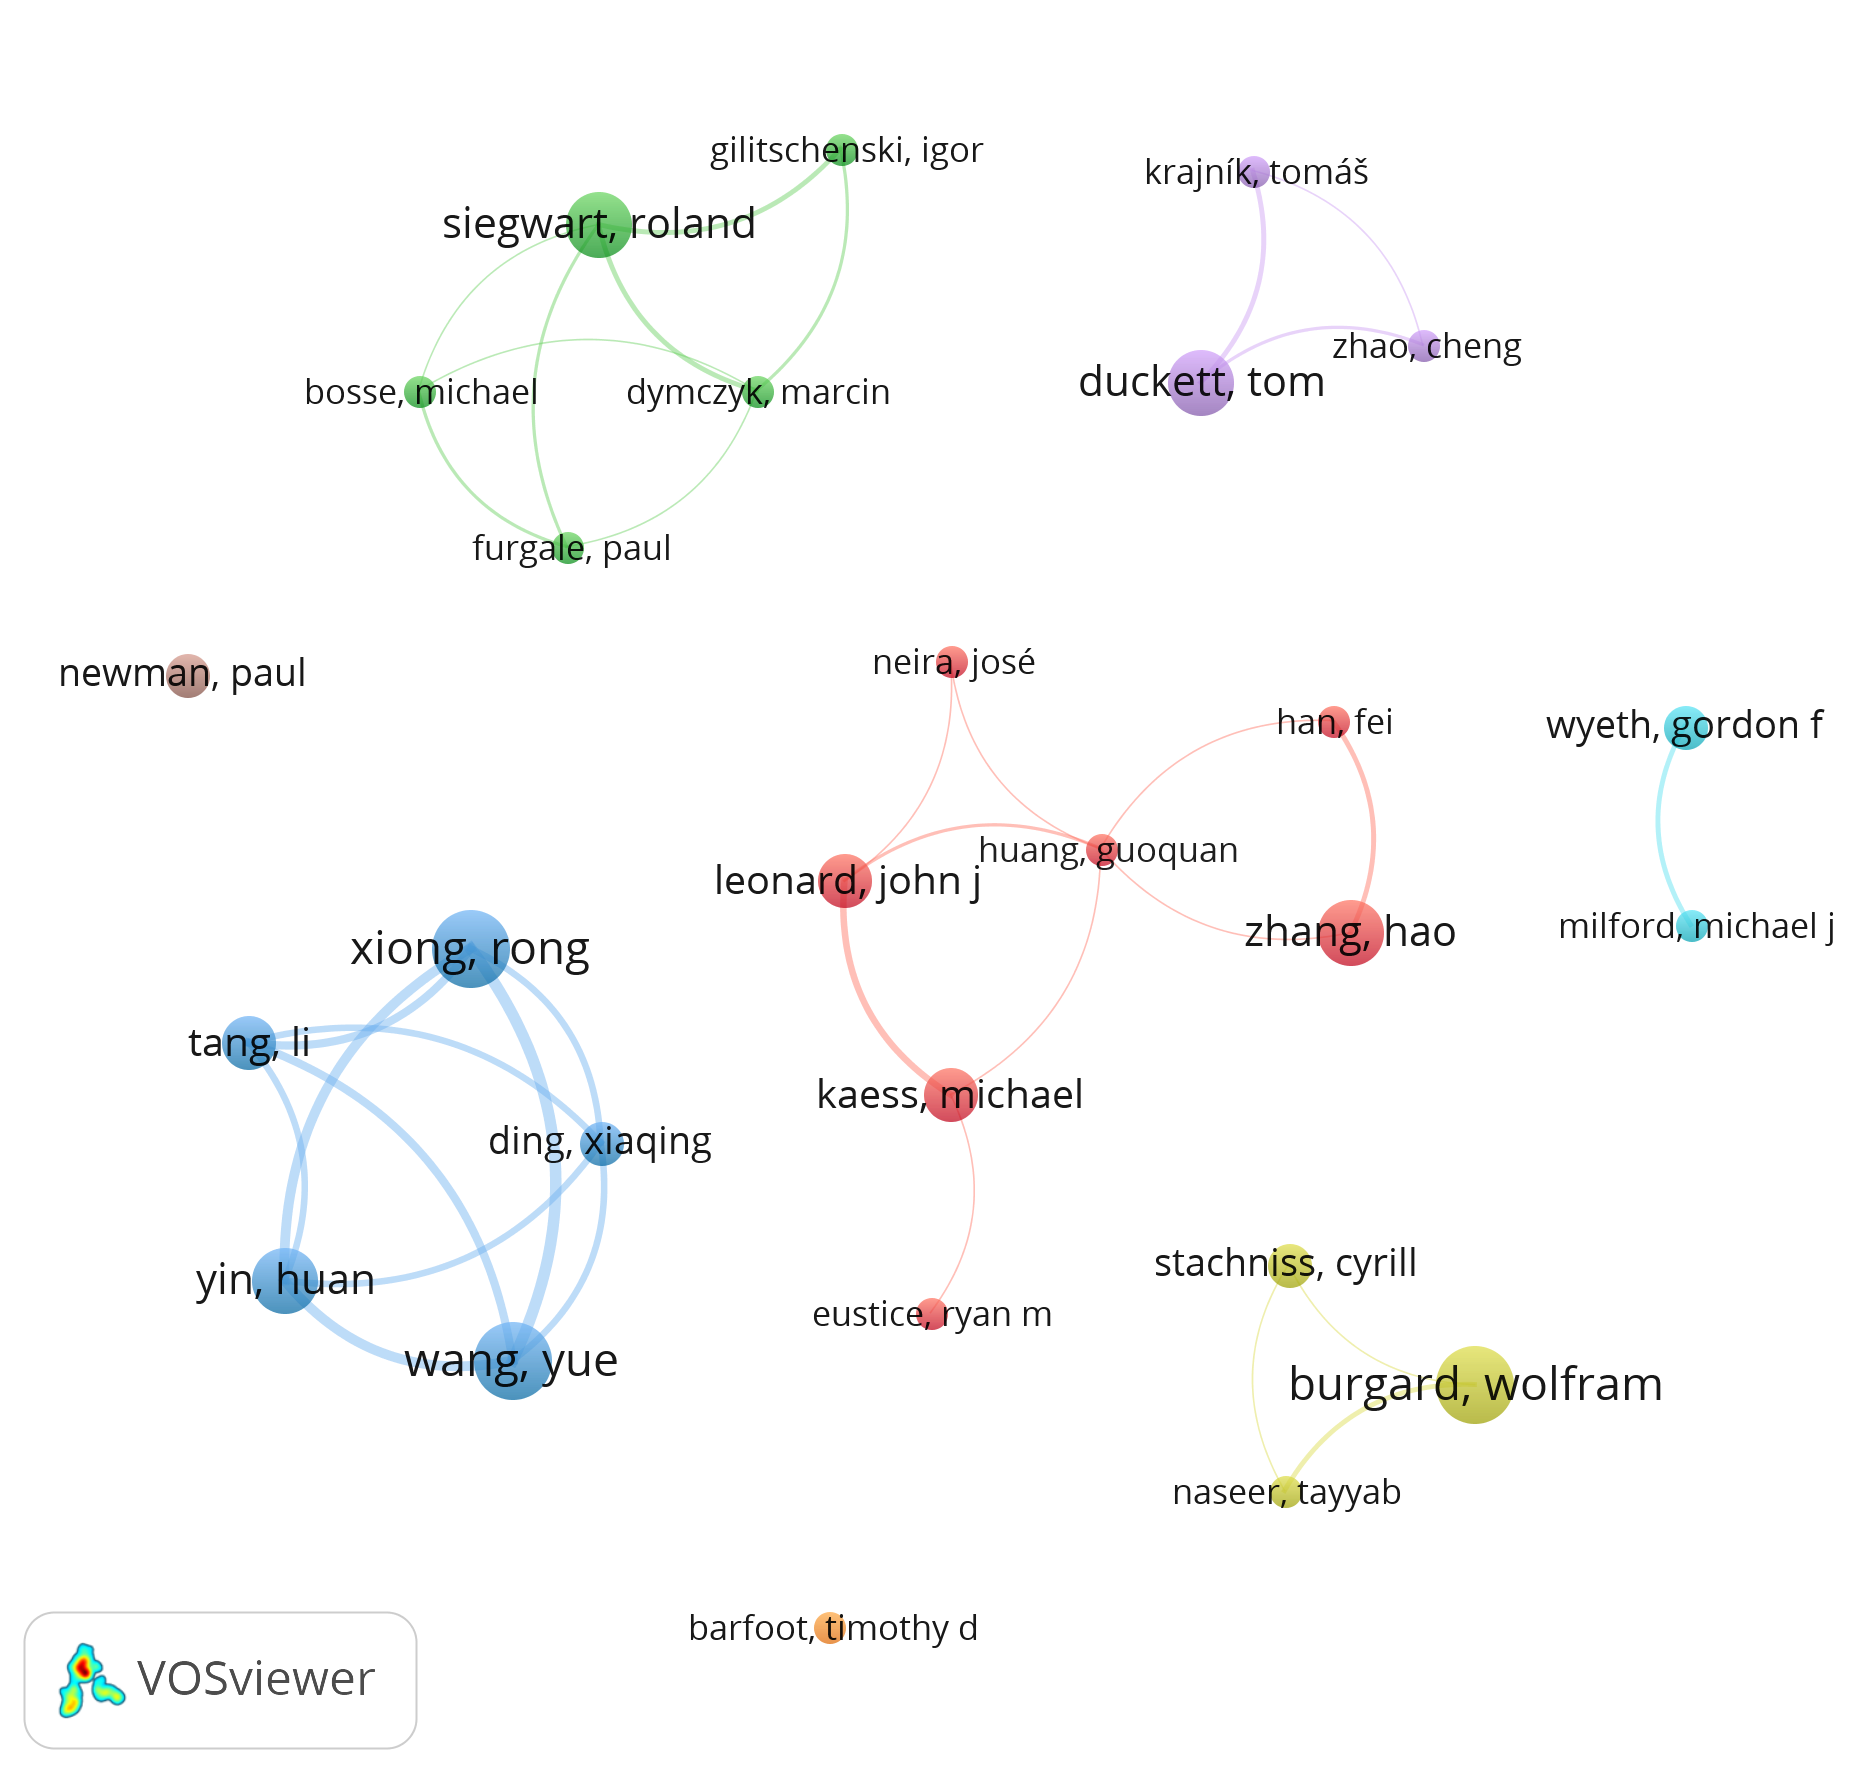
\includegraphics[width=\columnwidth]{figures/authors.png}
  \caption{Co-authorship analysis on the 142 included records generated by VOSviewer. Parameters used for generating the co-occurrence network: minimum number of occurrences = 3, attraction = 2, repulsion = -3, scale = 1.49, circles size variation = 1.0, lines size validation = 1.0.}
  \label{fig:overview:authors}
\end{figure}

Analyzing Figure~\ref{fig:overview:authors}, the co-authorship network presents 8 clusters. These clusters are separated from each other, i.e., no link exists between authors from different clusters. However, this separation does not mean that there is not any co-authorship between authors from different clusters only indicating that for a miminum of 3 co-authored documents there is not a connection between these 8 clusters. Even so, the graph presented in Figure~\ref{fig:overview:authors} allows the identification of the most relevant research networks in terms of number of co-authored documents and in the context of long-term localization and mapping, considering the 142 records included in this review. As a results, the following enumeration presents the authors that belong to each cluster in the format of author (number of co-authored documents):

\begin{enumerate}\setlength\itemsep{-0.5em}
\item Rong Xiong \orcid{0000-0001-9318-9014}\textsuperscript{,}\scholar{1hI9bqUAAAAJ} (7),
        Yue Wang \orcid{0000-0002-0981-935X}\textsuperscript{,}\scholar{N543LSoAAAAJ} (7),
        Huan Yin \orcid{0000-0002-0872-8202}\textsuperscript{,}\scholar{1fNc3vUAAAAJ} (6),
        Li Tang \orcid{0000-0003-2590-6872} (5),
        and Xiaqing Ding \orcid{0000-0001-7802-0130}\textsuperscript{,}\scholar{6u5OHUcAAAAJ} (4);
\item Hao Zhang \scholar{Ug2VxyUAAAAJ} (6),
        John J. Leonard \orcid{0000-0002-8863-6550}\textsuperscript{,}\scholar{WPe7vWwAAAAJ} (5),
        Michael Kaess \scholar{27eupmsAAAAJ} (5),
        Fei Han \orcid{0000-0002-8619-3987} (3),
        Guoquan Huang \scholar{trMUyZIAAAAJ} (3),
        José Neira \orcid{0000-0003-0668-977X}\textsuperscript{,}\scholar{scoMbR8AAAAJ} (3),
        and Ryan M. Eustice \orcid{0000-0002-9989-4942}\textsuperscript{,}\scholar{WroYmiAAAAAJ} (3);
\item Wolfram Burgard \orcid{0000-0002-5680-6500}\textsuperscript{,}\scholar{zj6FavAAAAAJ} (7),
        Cyrill Stachniss \orcid{0000-0003-1173-6972}\textsuperscript{,}\scholar{8vib2lAAAAAJ} (5),
        Giorgio Grisetti \orcid{0000-0002-8038-9989}\textsuperscript{,}\scholar{yD-SFG4AAAAJ} (3),
        Henrik Kretzschmar \scholar{pZuaUlwAAAAJ} (3),
        and Tayyab Naseer \orcid{0000-0002-3350-3005}\textsuperscript{,}\scholar{1FePZqEAAAAJ} (3);
\item Roland Siegwart \orcid{0000-0002-2760-7983}\textsuperscript{,}\scholar{MDIyLnwAAAAJ} (6),
        Igor Gilitschenski \orcid{0000-0001-6426-365X}\textsuperscript{,}\scholar{Nuw1Y4oAAAAJ} (3),
        Marcin Dymczyk \orcid{0000-0003-3667-8764}\textsuperscript{,}\scholar{XYHy7U8AAAAJ} (3),
        Michael Bosse \scholar{eopb1VgAAAAJ} (3),
        and Paul Furgale \orcid{0000-0002-7367-1046}\textsuperscript{,}\scholar{RNDtSG8AAAAJ} (3);
\item Tom Duckett \orcid{0000-0003-2971-7905}\textsuperscript{,}\scholar{et1GU2EAAAAJ} (6),
        Cheng Zhao \orcid{0000-0001-8502-3233}\textsuperscript{,}\scholar{EAC-8m0AAAAJ} (3),
        and Tomáš Krajník \orcid{0000-0002-4408-7916}\textsuperscript{,}\scholar{Qv3nqgsAAAAJ} (3);
\item Gordon F. Wyeth \orcid{0000-0002-4996-3612}\textsuperscript{,}\scholar{yfXZfXEAAAAJ} (5)
        and Michael J. Milford \orcid{0000-0002-5162-1793}\textsuperscript{,}\scholar{TDSmCKgAAAAJ} (4);
\item Paul Newman \scholar{BtO5fTUAAAAJ} (4);
\item Timothy D. Barfoot \orcid{0000-0003-3899-631X}\textsuperscript{,}\scholar{N_vPIhoAAAAJ} (3).
\end{enumerate}

When analyzing the affiliations of the authors mentioned previously at the time of publication, all authors of the first cluster belonged to the State Key Laboratory of Industrial Control and Technology (SKLICT) and the Institute of Cyber-Systems and Control at Zhejiang University in China. Even though Huan Yin, Yue Wang, Xiaqing Ding, Li Tang, and Rong Xiong mention their affiliation to the Joint Centre for Robotics Research between Zhejiang University, China, and the University of Technology Sydney, Sydney, in the work \parencite{yin-et-al:2020:2905046}, this specific affiliation only appeared in this article. The total link strength (sum of all links weights) of each of the authors in that cluster is higher than 16, meaning a high co-authorship between them. Indeed, all five authors have links between all of them.
Similar to the first cluster, the third, fourth, fifth, and sixth clusters have common affiliations within each one: the Autonomous Intelligent Systems at the University of Freiburg in Germany, the Autonomous Systems Lab (ASL) at ETH Zürich in Switzerland, the Lincoln Centre for Autonomous Systems (LCAS) at the University of Lincoln in UK, and the School of Electrical Engineering and Computer Science at Queensland University of Technology (QUT) in Australia.
However, the interlinking between the authors is not as strong as in the first cluster, as shown in Figure~\ref{fig:overview:authors} by the authors of these clusters not being connected between all the ones within each cluster. Even so, the common affiliation shows there is considerable interest by these research units in the long-term localization and mapping topic.

The affiliation analysis in the second cluster is more complex given that there was no affiliation common to all authors at the time of the records' publication. Instead, the following affiliations were found: Fei Han and Hao Zhang with the Department of Computer Science at Colorado School of Mines in the USA, Guoquan Huang with the Department of Mechanical Engineering at the University of Delaware in the USA, John J. Leonard and Michael Kaess with the Computer Science and Artificial Intelligence Laboratory (CSAIL) at the Massachusetts Institute of Technology (MIT) in the USA, Ryan M. Eustice with the Perceptual Robotics Laboratory (PeRL) at the University of Michigan in the USA, and José Neira with the Instituto Universitario de Investigación en Ingeniería de Aragón (I3A) at the Universidad de Zaragoza in Spain.
Although there are 5 different affiliations to which the 7 authors stated in the respective records, 4 of the research institutions noted for the second cluster are in the USA, indicating a possible reason for facilitating the linkage between these authors from different research units.

In terms of the clusters composed by single authors, the affiliations of Paul Newman and Timothy D. Barfoot are the Oxford Robotics Institute at the University of Oxford in UK and the Autonomous Space Robotics Laboratory (ASRL) at the University of Toronto Institute for Aerospace Studies (UTIAS) in Canada, respectively. Even though these two authors are not linked with any others in the network, the co-authorship analysis indicates that they have an interest in long-term localization and mapping. This interest is shown by their number of co-authored records: 4 and 3 by Paul Newman and Timothy D. Barfoot, respectively.

As for the number of co-authored publications, considering the 142 included records, the authors that appeared to have more research on the review's topic are Rong Xiong, Yue Wang, and Wolfram Burgard, given the 7 co-authored publications of each one. However, Rong Xiong and Yue Wang have co-authored the 7 documents attributed to each of them. This relation and similar ones can biase the analysis of which authors are having more impact in the review's topic.
The clustering shown in Figure~\ref{fig:overview:authors} allows a more unbiased analysis relative to the co-authorship links between authors. Thus, based on the clustering and which author from each cluster has the most co-authored publications, the most influential authors in long-term localization and mapping are the following ones: Rong Xiong (or Yue Wang), Hao Zhang, Wolfram Burgard, Roland Siegwart, Tom Duckett, Gordon F. Wyeth, Paul Newman, and Timothy D. Barfoot.

\subsection{Year of publication}
\label{sec:overview:year}

The relevance of the long-term localization and mapping topic can be evaluated by the evolution of the number of publications. Figure~\ref{fig:overview:year} presents this evolution from the earliest year of publication of the included records to the year at the time of writing this article. The latter has its respective data dashed to indicate that the last year is not completed at the time of writing. Analyzing Figure~\ref{fig:overview:year}, this review's topic seems to have gain relevance in 2009 with 6 works, compared to only one publication in 2007 and another in 2002 in the previous years to 2009. From that year onwards, the graph has an almost linear tendency reaching a maximum of 23 records in 2021, while already having 8 publications in 2022 until May 17, 2022. This tendency shows that long-term localization and mapping is gaining interest throughout the years and, consequently, supports the importance and relevance of this review for the scientific community.

\begin{figure}[!t]
  \centering
  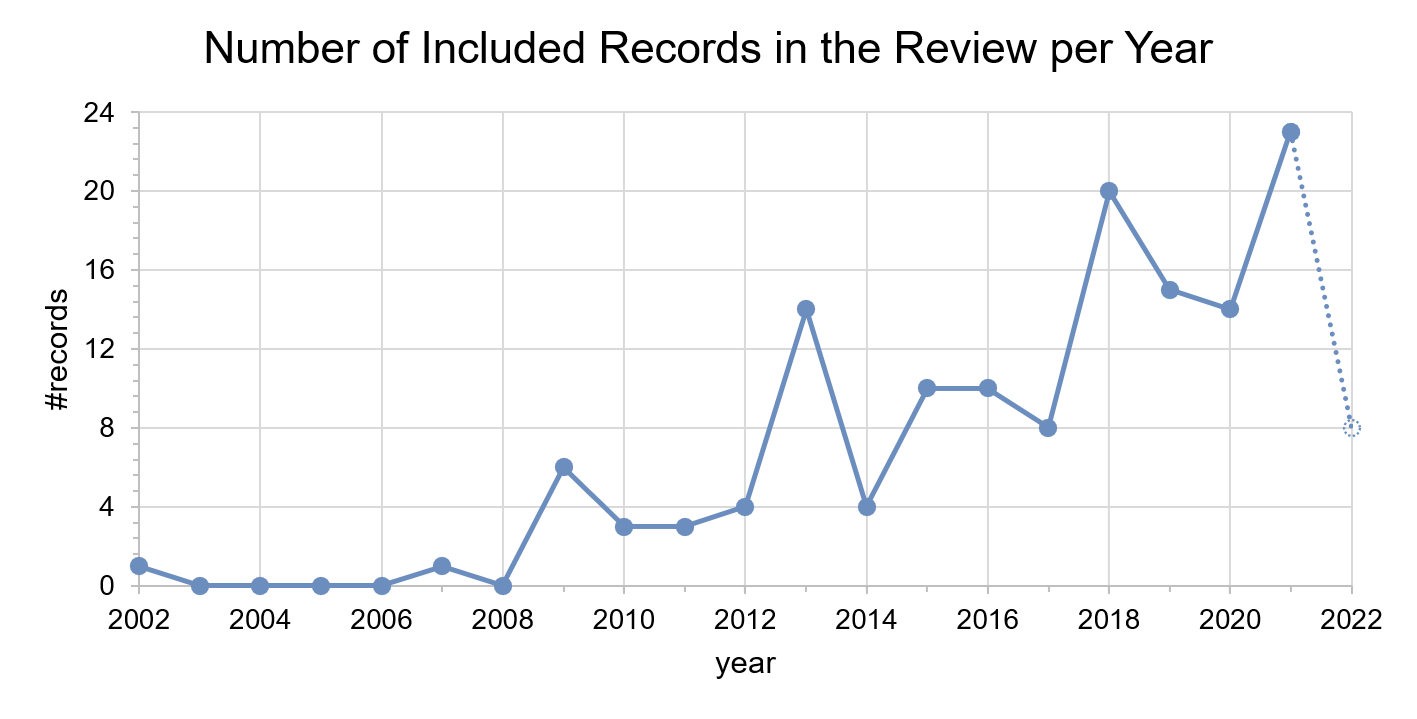
\includegraphics[width=\columnwidth]{figures/year.png}
  \caption{Evolution of published records per year considering the 142 included records in this review}
  \label{fig:overview:year}
\end{figure}

\subsection{Publication venue}
\label{sec:overview:publication}

Finally, the last overview of the 142 included records in the review is relative to the publication venue. Table~\ref{tab:overview:publication} presents the venues with more than 1 publication, separating the journals and conferences in two different tables (Tables~\ref{tab:overview:publication:journal} and \ref{tab:overview:publication:conference}, respectively).
The columns $\mu$ present the average year of publication of the records associated to a certain venue, while $\text{max}$ columns display the publishing recency by the year of the most recent publication in the venue. For comparing to the average value ($\mu$), the third column ($\sigma$) of each table presents the standard deviation based on the publication year data.
The last column state the number of records published in the venue from the 142 records included in the review for discussion.

\begin{table}[!h]
  \centering
  \caption{Publication venues of the included records in this review with more than one record published in the venue: (a) journals; (b) conferences. Legend: $\mu$ -- average year of publication, $\sigma$ -- standard deviation of the publication year, $\text{max}$ -- maximum year of publication, \# -- number of records published at a certain venue}
  \label{tab:overview:publication}
  \subfloat[][]{%
  \begin{tabular}{p{0.55\columnwidth}cccc}
\hline
                 & \multicolumn{3}{c}{\textbf{Year}} & \\
\cline{2-4}
\textbf{Journal} & $\mu$ & $\sigma$ & $\text{max}$ & \textbf{\#}\\
\hline
Robotics and Autonomous Systems & 2016 & 3.9 & 2021 & 13\\
IEEE Robotics and Automation Letters & 2019 & 1.7 & 2022 & 12\\
International Journal of Robotics Research & 2014 & 3.2 & 2022 & 11\\
Journal of Field Robotics & 2017 & 3.5 & 2022 & 8\\
Autonomous Robots & 2017 & 2.2 & 2020 & 7\\
IEEE Transactions on Intelligent Transportation Systems & 2021 & 0.8 & 2022 & 4\\
Sensors & 2019 & 0.8 & 2020 & 4\\
IEEE Transactions on Robotics & 2017 & 3.1 & 2022 & 4\\
IEEE Sensors Journal & 2020 & 1.5 & 2021 & 2\\
International Journal of Advanced Robotic Systems & 2020 & 1.5 & 2021 & 2\\
\hline
  \end{tabular}\label{tab:overview:publication:journal}%
  }
  \linebreak
  \subfloat[][]{%
  \begin{tabular}{p{0.55\columnwidth}cccc}
\hline
                    & \multicolumn{3}{c}{\textbf{Year}} & \\
\cline{2-4}
\textbf{Conference} & $\mu$ & $\sigma$ & $\text{max}$ & \textbf{\#}\\
\hline
IEEE International Conference on Robotics and Automation (ICRA) & 2016 & 3.9 & 2021 & 22\\
IEEE/RSJ International Conference on Intelligent Robots and Systems (IROS) & 2017 & 3.6 & 2021 & 17\\
IEEE International Conference on Robotics and Biomimetics (ROBIO) & 2019 & 2.1 & 2021 & 3\\
IEEE International Intelligent Transportation Systems Conference (ITSC) & 2018 & 2.4 & 2021 & 3\\
European Conference on Mobile Robots (ECMR) & 2014 & 0.9 & 2015 & 3\\
IEEE Intelligent Vehicles Symposium (IV) & 2019 & 0.5 & 2019 & 2\\
International Conference on 3D Vision (3DV) & 2018 & 1.5 & 2019 & 2\\
International Conference on Advanced Robotics (ICAR) & 2011 & 2.0 & 2013 & 2\\
\hline
  \end{tabular}\label{tab:overview:publication:conference}%
  }
\end{table}

In terms of journals, the Robotics and Autonomous Systems, IEEE Robotics and Automation Letters, and the International Journal of Robotics stand out with more than 10 publications. Also, these journals have a high standard deviation (greater than 1.5), indicating that the publications spread out throughout the years.
In the case of the IEEE Robotics and Automation Letters, these results gain more relevance indicating a recent trend on publishing on this journal, considering that its creation was only on 2015\footnote{\url{https://www.ieee-ras.org/publications/ra-l}}.
With more than 5 publications, the Journal of Field Robotics and the Autonomous Robots have recent average of publication (2017) with a high standard deviation (greater than 2.0), similarly indicating that authors have been publishing in these two journals along the years.
In contrast, the IEEE Transactions on Intelligent Transportation Systems and Sensors journals have a standard deviation lower than 1 year, with an average publication year of at least 2019. The recency of publication on these two journals with a very low deviation suggests a recent interest of the authors to publish in these two journals works related to long-term localization and mapping.

As for conferences, the data in Table~\ref{tab:overview:publication:conference} shows a high discrepancy in the number of publications related to this review's topic in ICRA and IROS compared to the other venues. Indeed, all the other conferences have only a maximum of 3 records published in them, compared to 22 and 18 papers in ICRA and IROS, respectively. When considering that 62 of the 142 included records are published in conferences, ICRA and IROS with a total of 40 published works related to this review's topic represent 65\% of works published in conferences and 27.8\% of all included records. This result expresses the high relevance of ICRA and IROS in the topic of long-term localization and mapping.

